\documentclass[11pt,a4paper]{article}
\usepackage[top=3cm, bottom=2cm, left=2cm, right=2cm]{geometry}
\usepackage[utf8]{inputenc}
\usepackage{amsmath, amsfonts, amssymb}
\usepackage{siunitx}
\usepackage[brazil]{babel}
\usepackage{graphicx}
\usepackage[margin=10pt,font={small, it},labelfont=bf, textfont=it]{caption}
\usepackage[dvipsnames, svgnames]{xcolor}
\DeclareCaptionFont{MediumOrchid}{\color[svgnames]{MediumOrchid}}
\usepackage[pdftex]{hyperref}
\usepackage{natbib}
\bibliographystyle{plainnat}
\bibpunct{[}{]}{,}{s}{}{}
\usepackage{color}
\usepackage{footnote}
\usepackage{setspace}
\usepackage{booktabs}
\usepackage{multirow}
\usepackage{subfigure}
\usepackage{fancyhdr}
\usepackage{leading}
\usepackage{indentfirst}
\usepackage{wrapfig}
\usepackage{mdframed}
\usepackage{etoolbox}
\usepackage[version=4]{mhchem}
\usepackage{enumitem}
\usepackage{caption}
\usepackage{titlesec}
\usepackage{tcolorbox}
\usepackage{tikz}
\usepackage{LobsterTwo}
\usepackage[T1]{fontenc}
\usepackage{fontspec}
\usepackage{txfonts}
\AtBeginEnvironment{equation}{\fontsize{13}{16}\selectfont}


\titleformat{\section}{\LobsterTwo\LARGE\color{CarnationPink}}{\thesection.}{1em}{}
\titleformat{\subsection}{\LobsterTwo\LARGE\color{CarnationPink}}{\thesubsection}{1em}{}


\DeclareCaptionLabelFormat{figuras}{\textcolor{DarkTurquoise}{Figura \arabic{figure}}}
\captionsetup[figure]{labelformat=figuras}

\makeatletter
\renewcommand\tagform@[1]{\maketag@@@{\color{CarnationPink}(#1)}}
\makeatother

\renewcommand{\theequation}{Eq. \arabic{equation}}
\renewcommand{\thefigure}{Fig. \arabic{figure}}
\renewcommand{\thesection}{\textcolor{CarnationPink}{\arabic{section}}}

\setlist[itemize]{label=\textcolor{CarnationPink}{$\mathbf{\square}$}}

\setlist[enumerate]{label=\textcolor{CarnationPink}{\arabic*.}, align=left}


\newcounter{exemplo}

\NewDocumentEnvironment{exemplo}{ O{} }{%
\allowbreak
\setlength{\parindent}{0pt}
  \begin{mdframed}[
  leftline=true,
  topline=false,
  rightline=false,
  bottomline=false,
  linewidth=2pt,
  linecolor=CarnationPink,
  frametitlerule=false,
  frametitlefont=\LobsterTwo\large\color{CarnationPink},
  frametitle={\color{CarnationPink}\LobsterTwo\large #1},
  ]
}{%
  \end{mdframed}
}

\setlength{\fboxsep}{5pt}
\setlength{\fboxrule}{1.5pt}
\usepackage{float}
\renewcommand{\thefootnote}{\alph{footnote}}
\usepackage{url}
\hypersetup{
	colorlinks=true,
	linkcolor=DarkTurquoise,
	filecolor=DarkTurquoise,      
	urlcolor=DarkTurquoise,
	citecolor=DarkTurquoise,
	pdftitle={Especialista em Física da Radioterapia}
}
\pagestyle{fancy}
\fancyhf{}
\renewcommand{\headrulewidth}{0pt}
\rfoot{Página \thepage}

\title{\LobsterTwo\Huge{Radiobiologia}}
\author{\LobsterTwo\Large{Mecanismos De Interação da Radiação e de Reparo do DNA}\nocite{*}}
\date{\LobsterTwo\textit{Dalila Mendonça}}
\begin{document}
	\maketitle


\section{Irradiação das Células}

	Quando as células são expostas à radiação ionizante, as interações iniciais ocorrem entre a radiação e os átomos ou moléculas dentro das células. O dano biológico subsequente às funções celulares é resultado dessas interações. O alvo primário para efeitos biológicos é o DNA, embora danos a outros componentes celulares também possam levar à morte celular. O dano celular pela radiação ionizante pode ocorrer por meio de ação direta ou indireta.

	Na ação direta, a radiação ionizante interage diretamente com o alvo crítico dentro da célula. Essa interação ocorre por meio de interações de Coulomb, onde a radiação pode ionizar (remover elétrons) ou excitar os átomos do alvo. Isso inicia uma cadeia de eventos físicos e químicos dentro da célula, resultando em dano biológico. A ação direta é particularmente importante quando partículas com alta transferência linear de energia (LET) interagem com o material biológico.

	Na ação indireta, a radiação ionizante interage com outras moléculas e átomos, principalmente a água presente dentro da célula (que constitui cerca de 80\% do conteúdo celular). Essa interação resulta na produção de radicais livres, que são espécies quimicamente reativas. Esses radicais livres podem se difundir dentro da célula e causar danos ao alvo crítico. Quando a radiação interage com a água, ela gera radicais livres altamente reativos, como o íon H2O+ (íon de água) e o radical \ce{OH^.} (radical hidroxila). Esses radicais livres podem causar danos ao alvo dentro da célula por meio de reações químicas.

	Os radicais livres gerados durante a ação indireta causam danos biológicos ao quebrar ligações químicas e induzir mudanças químicas nas células. Esses radicais livres são altamente reativos devido aos elétrons de valência não pareados. Aproximadamente dois terços do dano biológico causado por radiações de baixo LET, como raios X ou elétrons, são atribuídos à ação indireta. A ação indireta pode ser influenciada por sensibilizadores químicos (substâncias que aumentam a sensibilidade das células à radiação) ou protetores contra radiação (substâncias que protegem as células dos efeitos danosos da radiação).

	O processo de dano biológico por meio da ação indireta de raios X envolve as seguintes etapas:

	\begin{enumerate}
	\item A interação primária do fóton (efeito fotoelétrico, efeito Compton e produção de pares) produz um elétron de alta energia.
	\item O elétron de alta energia, ao se mover através do tecido, gera radicais livres na água.
	\item Os radicais livres têm o potencial de induzir alterações no DNA por meio da quebra de ligações químicas.
	\item As alterações nas ligações químicas levam, em última instância, a efeitos biológicos.
	\end{enumerate}

	A etapa 1 pertence ao domínio da física, a etapa 2 envolve a química, enquanto as etapas 3 e 4 estão no âmbito da radiobiologia.

	Quando uma célula é irradiada, pode resultar em um dos nove possíveis desfechos:

	\begin{enumerate}
		\item \textcolor{DarkTurquoise}{\textbf{Sem efeito:}} A irradiação não apresenta efeito discernível na célula.
		\item \textcolor{DarkTurquoise}{\textbf{Atraso na divisão:}} A célula experimenta um atraso em seu processo normal de divisão.
		\item \textcolor{DarkTurquoise}{\textbf{Apoptose:}} A célula morre antes de poder se dividir ou por fragmentação em corpos menores, que são então engolfados por células vizinhas.
		\item \textcolor{DarkTurquoise}{\textbf{Falha reprodutiva:}} A célula morre ao tentar a primeira ou subsequente mitose (divisão celular).
		\item \textcolor{DarkTurquoise}{\textbf{Instabilidade genômica:}} Há uma forma retardada de falha reprodutiva causada por instabilidade genômica induzida.
		\item \textcolor{DarkTurquoise}{\textbf{Mutação:}} A célula sobrevive, mas adquire uma mutação genética.
		\item \textcolor{DarkTurquoise}{\textbf{Transformação:}} A célula sobrevive, mas a mutação adquirida leva a um fenótipo transformado, potencialmente resultando em carcinogênese (desenvolvimento de câncer).
		\item \textcolor{DarkTurquoise}{\textbf{Efeitos em células vizinhas (Bystander effect):}} Uma célula irradiada pode liberar sinais que afetam células vizinhas não irradiadas, induzindo danos genéticos nessas células.
		\item \textcolor{DarkTurquoise}{\textbf{Respostas adaptativas:}} A célula irradiada passa por estímulo e desenvolve resistência aumentada à subsequente irradiação, exibindo uma resposta adaptativa.
	\end{enumerate}


\section{Tipos de Dano ao DNA}

	A oxidação, a quimioterapia e a radioterapia podem danificar o DNA e há muitas maneiras pelas quais isso pode ocorrer.

	\begin{itemize}[label=\textcolor{CarnationPink}{$\blacktriangleright$}]
		\item \textcolor{DarkTurquoise}{\textbf{Dano à base: }} Um dano à base do DNA ocorre quando uma das bases nitrogenadas (adenina, timina, citosina ou guanina) que compõem a sequência de DNA é alterada ou modificada de de modo que essa base do é quimicamente alterada. Quando ocorre um dano à base do DNA e esse dano não é corrigido adequadamente, podem ocorrer erros de replicação e mutações pontuais ou predispor a danos adicionais no DNA.
		
		\item \textcolor{DarkTurquoise}{\textbf{Desparidade de Bases (Base Mismatch):}} Durante a replicação, as cadeias de DNA são duplicadas, e cada base em uma das cadeias é pareada com uma base complementar na nova cadeia em formação. No entanto, às vezes ocorre um erro e uma base incorreta é inserida na nova cadeia. Esse erro é chamado de "base mismatch" ou "desparidade de bases". Significa que uma base incorreta é emparelhada com outra base na nova cadeia de DNA. Essa desparidade pode levar a uma mutação pontual, que é uma alteração em apenas um par de bases no DNA. Se o erro não for corrigido pelo sistema de reparo do DNA, a mutação pontual pode persistir e ser transmitida para as células descendentes. Dependendo da localização e do efeito da mutação, ela pode ter diferentes consequências, como alterar a sequência de aminoácidos em uma proteína, interferir na função da proteína ou ter outros efeitos na expressão gênica.
		
		\item \textcolor{DarkTurquoise}{\textbf{Dímeros de pirimidina:}} Os dímeros de pirimidina são danos específicos que ocorrem no DNA quando duas bases de pirimidina adjacentes são ligadas covalentemente entre si. Geralmente, esse tipo de dano ocorre entre duas bases de timina (T), embora também possa ocorrer entre uma timina (T) e uma citosina (C). Esses danos são causados principalmente pela exposição à radiação ultravioleta (UV), como a luz solar. A formação de dímeros de pirimidina causa distorções na estrutura da dupla hélice de DNA. Essas distorções podem interferir na replicação do DNA, na transcrição de genes e na reparação do DNA. Os dímeros de pirimidina impedem a ação correta das enzimas envolvidas nesses processos, afetando assim a integridade e a estabilidade do genoma. Quando o DNA danificado com dímeros de pirimidina é replicado, a replicação ocorre de maneira incorreta nas regiões danificadas. Isso resulta em mutações pontuais, que são alterações em um único par de bases do DNA. Essas mutações podem ter consequências importantes, pois podem afetar a função de genes específicos e contribuir para o desenvolvimento de doenças, como câncer de pele.
		
    \item \textcolor{DarkTurquoise}{\textbf{Intercalação:}} A intercalação de DNA é um tipo de dano que ocorre quando moléculas ou compostos químicos se inserem entre as bases nitrogenadas da dupla hélice do DNA. Essas moléculas "intercalantes" são geralmente planas e hidrofóbicas, permitindo que se encaixem entre as bases adjacentes do DNA. A intercalação causa uma perturbação na estrutura normal da dupla hélice do DNA, resultando em uma expansão localizada na hélice. Essa expansão pode levar a uma série de efeitos, incluindo alterações nas propriedades físicas e químicas do DNA. As moléculas intercalantes podem ser compostos naturais ou sintéticos, e muitas vezes são produtos químicos que podem ser encontrados no ambiente, como certos corantes, medicamentos e substâncias presentes na fumaça do cigarro. Alguns exemplos comuns de compostos intercalantes são a etidiuma brometo, proflavina, daunorrubicina e doxorrubicina. Isso pode impedir a função e a replicação do gene.
    
    \item \textcolor{DarkTurquoise}{\textbf{Crosslinking:}} Crosslinking (ou reticulação) do DNA é um tipo de dano em que as duas cadeias de DNA são ligadas entre si, formando uma ligação covalente anormal. Essas ligações cruzadas podem ocorrer entre duas bases adjacentes na mesma cadeia de DNA (crosslinking intrafilamentar) ou entre bases em cadeias de DNA diferentes (crosslinking interfilamentar). O crosslinking pode ser causado por diversos agentes químicos e físicos, como agentes alquilantes, radiação ionizante e certos medicamentos. Esses agentes induzem a formação de ligações covalentes entre as bases do DNA ou entre o DNA e outras moléculas presentes no ambiente celular. O dano por crosslinking é particularmente problemático porque impede a separação das duas cadeias de DNA, necessária para processos como replicação, transcrição e reparo. Isso pode levar a bloqueios no fluxo normal das informações genéticas e comprometer a funcionalidade das células. Isso pode impedir a função e a replicação do gene ou causar quebras na fita de DNA.
    
    \item \textcolor{DarkTurquoise}{\textbf{Single-Strand Breaks (SSBs):}} As quebras de fita única são danos no DNA em que apenas uma das duas cadeias da molécula de DNA é interrompida, resultando em uma quebra na estrutura da fita de DNA. Nesse tipo de dano, apenas uma das fitas de DNA é rompida. Isso resulta em uma separação das bases na fita danificada, enquanto a outra fita permanece intacta. Isso é facilmente reparado, desde que a outra fita ainda esteja intacta.
    
    \item \textcolor{DarkTurquoise}{\textbf{Double-Strand Breaks (DSBs):}} Uma quebra de fita dupla é um tipo de dano no DNA em que ambas as fitas da dupla hélice do DNA são rompidas em locais próximos ou em regiões distintas da molécula de DNA. As extremidades nas quebras serão “pegajosas” e podem reagir com outras fitas de DNA quebradas “pegajosas”. Isso causa aberrações cromátides e cromossômicas que podem ser mutagênicas ou letais. É considerada uma das formas mais graves de dano ao DNA. Quando ocorrem quebras de fita dupla, há a perda da continuidade da dupla hélice e interrupção do fluxo normal de informações genéticas.
	\end{itemize}

\section{Danos ao DNA causados Pela Radiação Ionizante}

	Cada Gy de radiação ionizante (raios-x) causa aproximadamente:

	\begin{itemize}[label=\textcolor{CarnationPink}{$\blacktriangleright$}]
		\item $>$ 2000 danos à bases;
		\item 30 crosslinking DNA-DNA;
		\item 1000 SSbs; e
		\item 40 - DSBs.
	\end{itemize}

	\textcolor{MediumOrchid}{\textbf{A DSB é o principal mecanismo de morte celular após a exposição à radiação ionizante}, de modo que é possível correlacionar o número de DSBs com a morte celular, o que não é p}ossível ser feito com outros tipos de dano. Por outro lado, o dano ao DNA induzido por quimioterapia depende da droga administrada e pode incluir danos à base, intercalação, reticulação e quebras duplas. 

	A radiação ionizante pode formar aglomerados de pares de íons na água, como mostra a \ref{fig:spurEBlob}. “Spurs” contêm 3 pares de íons em $\sim$ 4 nm e predominam após a exposição à irradiação de baixo LET. “Blobs” contêm 12 pares de íons em $\sim$ 7 nm e predominam após a exposição à irradiação de alto LET.

	\begin{figure}[h]
		\centering
		\fcolorbox{DarkTurquoise}{white}{%
			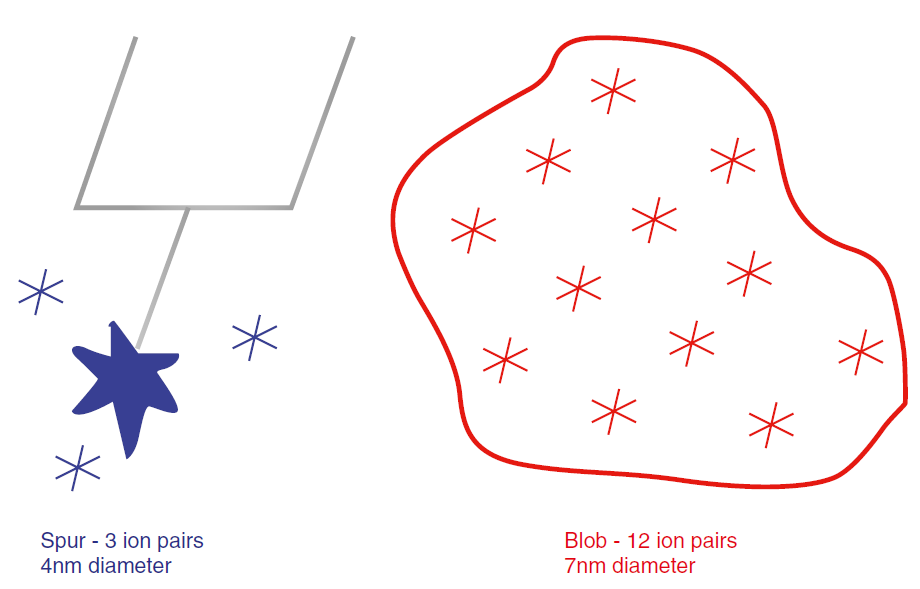
\includegraphics[width=0.8\textwidth]{Imagens/spurEBlob.png}
		}%
		\caption{Aglomerados de pares de íons causados pela radiação ionizante}
		\label{fig:spurEBlob}
	\end{figure}

	Regiões com múltiplos danos locais são definidos como lesões múltiplas no DNA, próxima umas das outras, como mostra a \ref{fig:dbsRadioInduzisd}. Os dano a base e as SSBs são facilmente reparados quando sozinhos, mas podem ser muito difíceis de reparar se agrupados. Duas SSBs próximas uma da outra provavelmente se tornarão uma DSB.

	\begin{figure}[h]
		\centering
		\fcolorbox{DarkTurquoise}{white}{%
			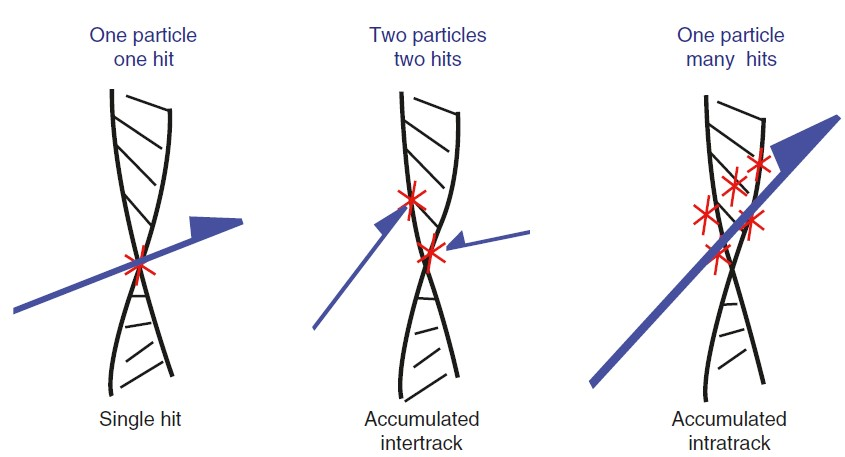
\includegraphics[width=0.8\textwidth]{Imagens/dbsRadioInduzisd.jpg}
		}%
		\caption{Quebras Duplas Raio-induzidas.}
		\label{fig:dbsRadioInduzisd}
	\end{figure}


\section{Acertos Únicos e Dano Acumulado}

	Conceitualmente, existem várias maneiras de ocorrer dano letal (DSBs). Por exemplo:

	\begin{itemize}[label=\textcolor{CarnationPink}{$\blacksquare$}]
		\item \textcolor{DarkTurquoise}{\textbf{Single Hit e Intra-track Acumulado:}} O dano é causado por uma única partícula. O número de DSBs formadas por este mecanismo é determinado pela dose total, mas não pela taxa de dose. Portanto, essas lesões são mais prováveis com irradiação de alto LET.
		\item \textcolor{DarkTurquoise}{\textbf{Inter-track Acumulado:}} O dano é causado por duas partículas separadas, como duas SSBs combinados em uma DSB. O número de DSBs formadas por este mecanismo é determinado pela dose total e taxa de dose. Com irradiação de baixa taxa de dose, o reparo do DNA pode impedir que danos não-DSB se transformem em DSBs.
	\end{itemize}

\section{Aberrações de Cromátides e Cromossômicas}

	Aberrações são mutações grosseiras criadas por quebras de fita dupla. O DNA quebrado é pegajoso e se não forem reparados ou mal reparados, os fragmentos de DNA ficarão juntos na ordem errada. As aberrações podem ser de cromátides ou cromossômicas e alguns tipos de aberrações podem ser cromossômicas ou cromátides, enquanto outras são limitadas a um tipo.

	A aberração de cromátide refere-se a alterações estruturais que ocorrem dentro de uma única cromátide, que é uma das duas cópias idênticas resultantes da replicação de um cromossomo antes da divisão celular.  Essas alterações podem incluir deleções (perda de parte do cromossomo), duplicações (repetições de partes do cromossomo), inversões (rearranjos na orientação das seções do cromossomo) e translocações (troca de segmentos entre cromossomos não homólogos). 

	Já a aberração cromossômica refere-se a alterações estruturais ou numéricas que afetam um ou mais cromossomos inteiros. Uma aberração ocorre em um cromossomo não replicado. Quando o cromossomo é replicado, a aberração é idêntica em ambas as cromátides. As alterações estruturais podem envolver deleções, duplicações, inversões e translocações, semelhantes às aberrações de cromátide. Além disso, as aberrações cromossômicas também podem envolver perdas ou ganhos de cromossomos inteiros, resultando em alterações no número total de cromossomos (aneuploidia) ou em rearranjos estruturais extensos.



\subsection{Aberrações Instáveis}

	As aberrações instáveis referem-se a alterações cromossômicas que podem ocorrer de maneira transitória ou reversível. Essas alterações estão sujeitas a mudanças ao longo do tempo e podem ser revertidas durante o processo de divisão celular ou reparo do DNA. Porém, Uma aberração instável diminui em número ao longo do tempo porque é altamente provável que cause morte celular pois essas aberrações impedem que os cromossomos se segreguem adequadamente durante a mitose.

\subsection*{Aberração Dicêntrica}


	As aberrações dicêntricas são um tipo de anormalidade cromossômica estrutural que ocorre quando dois cromossomos não homólogos se unem por meio de seus centrômeros. Essa fusão anormal resulta em um cromossomo com dois centrômeros e duas regiões de braços cromossômicos que se estendem em direções opostas, como mostra a \ref{fig:aberracaoDicentrica}. 

	\begin{wrapfigure}{r}{0.5\textwidth}
		\fcolorbox{DarkTurquoise}{white}{%
			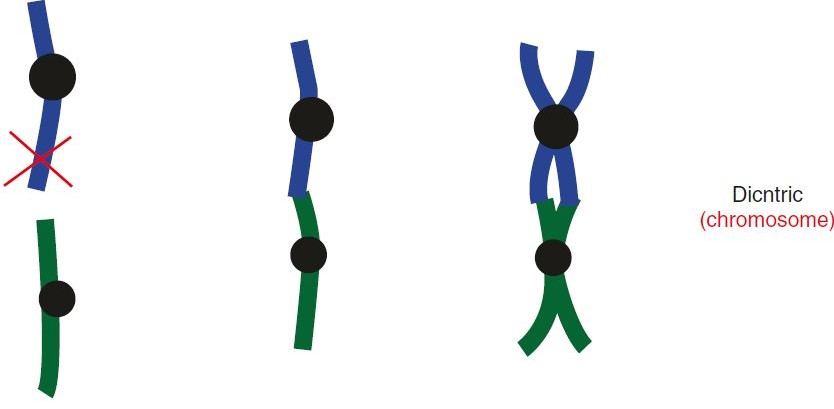
\includegraphics[width=0.48\textwidth]{Imagens/aberracaoDicentrica.JPG}
		}%
		\caption{Aberração dicêntrica (cromossomo)}
		\label{fig:aberracaoDicentrica}
	\end{wrapfigure}
	
	Geralmente, os centrômeros são os pontos de ancoragem para a segregação adequada dos cromossomos durante a divisão celular. No entanto, nas aberrações dicêntricas, a presença de dois centrômeros cria uma situação complexa, na qual as forças de segregação puxam em direções opostas. Isso pode resultar em instabilidade durante a divisão celular, causando problemas na segregação cromossômica e na distribuição correta do material genético para as células filhas. Durante a divisão celular subsequente, esses cromossomos dicêntricos podem se romper, resultando em quebras cromossômicas e reorganizações adicionais. Além disso, a formação de uma ponte cromossômica entre os dois centrômeros pode levar a problemas na separação dos cromossomos durante a divisão celular, causando desequilíbrios genéticos nas células filhas. Essas anormalidades cromossômicas podem levar a defeitos no desenvolvimento, distúrbios genéticos e câncer.

\subsection*{Anel}

	A anomalia cromossômica do tipo anel refere-se a uma alteração estrutural dos cromossomos na qual uma porção do cromossomo se perde e os dois extremos restantes se unem para formar uma estrutura em forma de anel. Nesse caso, o cromossomo não possui extremidades distintas, mas sim um anel fechado, como mostra a \ref{fig:aberracaoAnel}.

	\begin{wrapfigure}{l}{0.5\textwidth}
		\fcolorbox{DarkTurquoise}{white}{%
			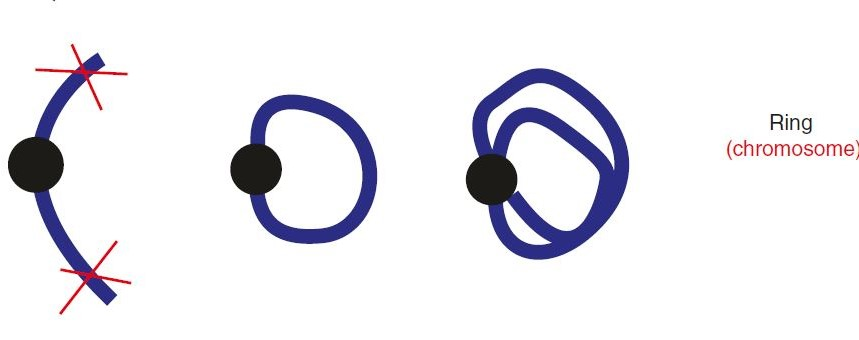
\includegraphics[width=0.48\textwidth]{Imagens/aberracaoAnel.JPG}
		}%
		\caption{Anel (cromossomo)}
		\label{fig:aberracaoAnel}
	\end{wrapfigure}	

	Essa anomalia ocorre quando ocorrem quebras em ambos os braços de um cromossomo e as extremidades livres se unem para formar o anel. A porção do cromossomo que está dentro do anel pode ser perdida, resultando em uma perda de material genético. Dependendo da região do cromossomo envolvida e dos genes afetados, a anomalia do anel cromossômico pode ter diferentes consequências clínicas e sintomas associados. Os anéis cromossômicos podem ocorrer em vários cromossomos, mas são mais comumente observados nos cromossomos acrocêntricos, como o 13, 14 e 15.
	
	Essa anomalia cromossômica geralmente ocorre de forma esporádica, ou seja, não é herdada dos pais. No entanto, em alguns casos, pode ocorrer transmissão hereditária. As consequências clínicas da anomalia do anel cromossômico podem variar amplamente. Algumas pessoas com essa anomalia podem não apresentar sintomas significativos, enquanto outras podem apresentar atraso no desenvolvimento, deficiência intelectual, problemas de crescimento, malformações congênitas, distúrbios do espectro autista e outras características clínicas específicas. O impacto e a gravidade das anomalias do anel cromossômico podem depender do tamanho e da composição genética da região perdida dentro do anel.


\subsection*{Ponte de Anáfase}

	A anomalia de ponte de anáfase, também conhecida como ponte anafásica, é uma anomalia cromossômica que ocorre durante a divisão celular chamada anáfase. A anáfase é a fase do ciclo celular em que os cromossomos duplicados são separados e puxados para polos opostos da célula. Nas células normais, durante a anáfase, os cromossomos são puxados em direções opostas por estruturas chamadas microtúbulos do fuso mitótico. No entanto, na presença de uma anomalia de ponte de anáfase, ocorre uma ligação anormal entre cromossomos ou fragmentos cromossômicos separados.

	\begin{wrapfigure}{r}{0.5\textwidth}
		\fcolorbox{DarkTurquoise}{white}{%
			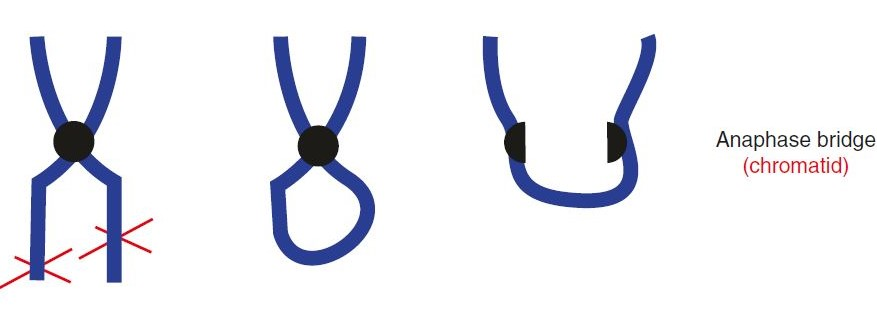
\includegraphics[width=0.48\textwidth]{Imagens/ponteDeAnafase.JPG}
		}%
		\caption{Ponte de Anáfase (cromátide)}
		\label{fig:ponteDeAnafase}
	\end{wrapfigure}

	Essas pontes anafásicas são formadas quando ocorre uma quebra do DNA em diferentes cromossomos ou segmentos cromossômicos, e as extremidades livres se ligam ou se fundem, formando uma conexão entre os cromossomos, como mostra a \ref{fig:ponteDeAnafase}. Essas pontes podem ocorrer devido a erros na replicação do DNA, danos ao DNA, falhas nos mecanismos de reparo do DNA ou outras condições que afetam a integridade cromossômica como a radiação ionizante.

	Durante a anáfase, pode-se observar visualmente a presença de estruturas de ponte que conectam os cromossomos ou fragmentos cromossômicos. As pontes anafásicas podem interferir na correta segregação dos cromossomos, levando a atrasos na separação dos cromossomos para os polos opostos da célula e também podem levar a quebras cromossômicas adicionais, resultando em rearranjos cromossômicos complexos. A presença de pontes anafásicas e as quebras cromossômicas associadas podem levar a perdas ou ganhos de material genético, causando desequilíbrios genéticos nas células filhas.

\subsection{Aberrações Estáveis}

	As aberrações estáveis são alterações cromossômicas que são passadas para as células filhas durante a divisão celular e são mantidas de forma estável ao longo do tempo. Essas alterações não são facilmente corrigidas ou revertidas pelo reparo do DNA e podem persistir nas células e em gerações subsequentes. Ou seja, uma aberração estável pode persistir por anos porque é pouco provável que cause morte celular uma vez que não afeta a segregação dos cromossomos durante a mitose.

\subsection*{Deleção}

	A deleção é uma aberração cromossômica que ocorre quando uma porção do DNA é perdida de um cromossomo. Isso significa que um segmento do cromossomo é apagado ou ausente, como mostra a \ref{fig:delecao}.
	
	\begin{wrapfigure}{l}{0.5\textwidth}
		\fcolorbox{DarkTurquoise}{white}{%
			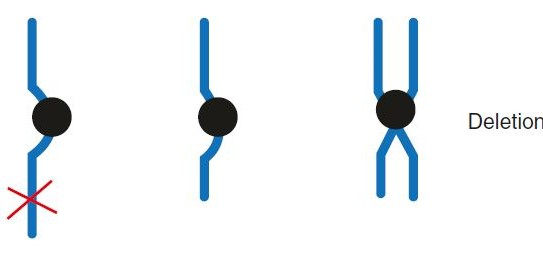
\includegraphics[width=0.48\textwidth]{Imagens/delecao.JPG}
		}%
		\caption{Deleção}
		\label{fig:delecao}
	\end{wrapfigure}
	
	A principal característica das deleções é a perda de uma porção do DNA cromossômico. Isso pode resultar na ausência de genes específicos, levando a alterações na expressão gênica e potenciais efeitos fenotípicos, o que caracteriza a perda de material genético. Em muitos casos, a deleção causa um rearranjo estrutural no cromossomo, pois as extremidades do cromossomo podem se unir para fechar a lacuna deixada pela deleção. Isso pode resultar em uma forma alterada ou encurtada do cromossomo. Devido à perda de genes, as deleções podem levar a desequilíbrios gênicos, especialmente se a deleção afetar regiões que contêm genes essenciais. O desequilíbrio gênico pode resultar em alterações no desenvolvimento, funcionamento celular ou metabólico.

	Os efeitos das deleções podem variar amplamente, dependendo do tamanho e dos genes envolvidos. Algumas deleções podem ser assintomáticas ou ter efeitos mínimos, enquanto outras podem estar associadas a condições genéticas específicas, deficiências intelectuais, anomalias congênitas ou distúrbios do desenvolvimento. Em alguns casos, as deleções cromossômicas podem ser herdadas dos pais. Isso ocorre quando um dos pais possui uma deleção em um dos cromossomos e a transmite para a prole. No entanto, muitas deleções ocorrem de forma espontânea e não são hereditárias.

\subsection*{Translocação Simétrica}

	A translocação simétrica é um tipo específico de aberração cromossômica em que dois cromossomos diferentes trocam segmentos de material genético de forma recíproca e equilibrada. Isso significa que uma porção de um cromossomo é transferida para outro cromossomo, enquanto uma porção correspondente é transferida de volta para o cromossomo original.

	\begin{wrapfigure}{r}{0.5\textwidth}
		\fcolorbox{DarkTurquoise}{white}{%
			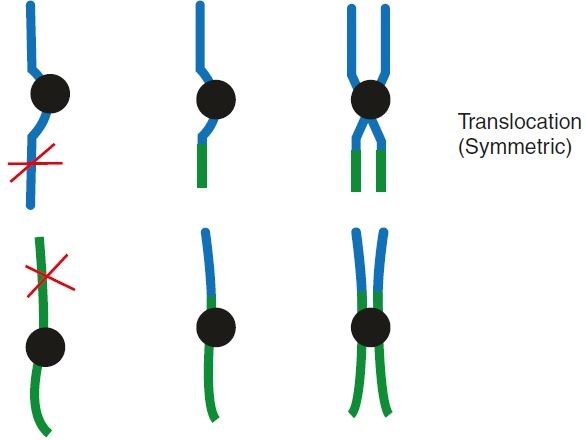
\includegraphics[width=0.48\textwidth]{Imagens/translocacaoSimetrica.JPG}
		}%
		\caption{Translocação Simétrica	}
		\label{fig:translocacaoSimetrica}
	\end{wrapfigure}

	A \ref{fig:translocacaoSimetrica} exemplifica a translocação simétrica. De modo geral, na translocação simétrica, ocorre uma troca recíproca de material genético entre dois cromossomos. Isso significa que as porções envolvidas nos cromossomos são trocadas em ambas as direções, resultando em uma troca equilibrada de material genético. A translocação simétrica resulta então em um rearranjo estrutural dos cromossomos envolvidos onde as extremidades dos cromossomos se unem para permitir a troca de segmentos, formando uma nova configuração estrutural.
	
	Ao contrário de algumas aberrações cromossômicas, como deleções ou duplicações, em que ocorre perda ou ganho de material genético, a translocação simétrica preserva a quantidade total de DNA. Isso significa que não há perda ou ganho líquido de material genético envolvido nessa aberração. Porém, embora a translocação simétrica em si não resulte em perda ou ganho de material genético, ela pode causar desequilíbrios genéticos nas células filhas durante a divisão celular. Isso ocorre porque a translocação simétrica pode afetar a separação correta dos cromossomos durante a divisão celular, levando à produção de células com conteúdo cromossômico anormal.

	Além da translocação simétrica, existem outros tipos de translocação cromossômica, incluindo:

	\begin{itemize}
		\item Translocação recíproca: Nesse tipo de translocação, dois cromossomos diferentes trocam segmentos de material genético de forma não equilibrada. Isso pode resultar em perda ou ganho líquido de material genético e potencialmente levar a desequilíbrios genéticos.
		\item Translocação robertsoniana: Nessa forma de translocação, dois cromossomos acrocêntricos (cromossomos com centrômeros localizados perto das extremidades) se fundem para formar um cromossomo maior. Esse tipo de translocação está associado a condições como a Síndrome de Down (trissomia do cromossomo 21).
	\end{itemize}


\section{Curva Linear-Quadratica para avaliar a Dose-Resposta}

	Ao avaliar graficamente o dano do DNA em função da dose fornecida que causa este dano, obtém-se uma curva ascendente com a forma linear-quadrática, como mostra a \ref{fig:DbsLinearQuadratico}.

	\begin{figure}[h]
		\centering
		\fcolorbox{DarkTurquoise}{white}{%
			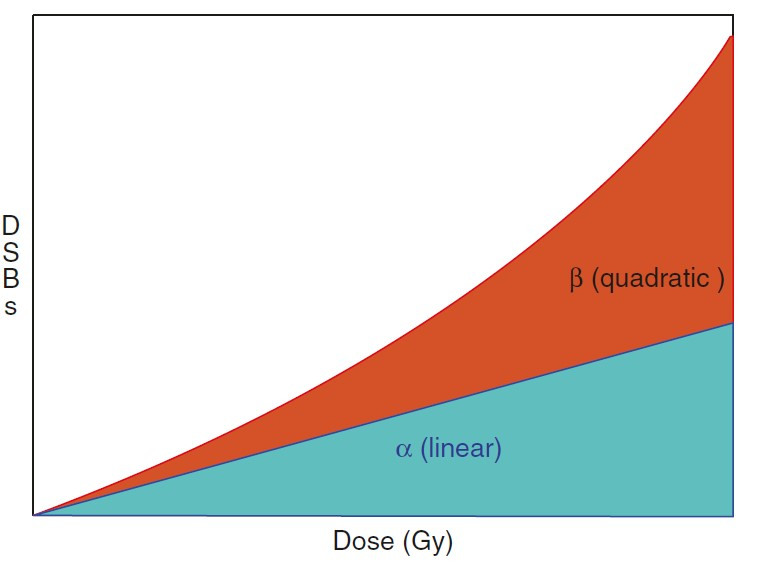
\includegraphics[width=0.5\textwidth]{Imagens/DbsLinearQuadratico.jpg}
		}%
		\caption{Curva Linear-Quadrática. A produção de DSB nas células é uma função linear-quadrática da dose. O número total de DSBs pode ser expresso pela soma do dano ``linear'' (independente do tamanho do fracionamento) e do dano ``quadrático'' (dependente do fracionamento)}
		\label{fig:DbsLinearQuadratico}
	\end{figure}

	O dano linear é diretamente proporcional a dose e é avaliado pelo coeficiente linear $\alpha$. Este dano é representado pelo dano de único acerto e o dano acumulado intra-track, no qual são completamente independentes do tamanho do fracionamento ou da taxa de dose. 

	O dano quadrático é proporcional ao quadrado da dose e é avaliado pelo coeficiente quadrático $\beta$.  Este dano é devido ao dano acumulado inter-track que é fortemente dependente do tamanho do fracionamento e da taxa de dose.

	Essa curva é a lógica por trás do modelo linear-quadrático $(\alpha/\beta)$ de sobrevivência celular e permite avaliar a quantidade de aberrações formadas em função da dose entregue. A \ref{fig:aberracaoEDose} mostra frequência de aberrações cromossômicas (dicêntricas e aneis) que são uma função linear-quadrática com a dose porque as aberrações são consequências de interações de duas quebras separadas. A baixas doses, ambas as quebras podem ser causadas pelo mesmo elétrons, portanto a probabilidade de uma aberração de permutação é proporcional à dose (D). Em altas doses, as duas quebras são causadas preferencialmente por elétrons separados e, portanto, a probabilidade de uma aberração de permutação é proporcional ao quadrado da dose ($D^2$).

	\begin{figure}[h]
		\centering
		\fcolorbox{DarkTurquoise}{white}{%
			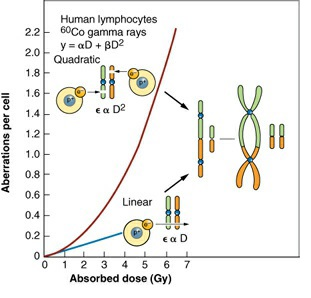
\includegraphics[width=0.5\textwidth]{Imagens/aberracaoEDose.jpg}
		}%
		\caption{Aberrações em Função da dose}
		\label{fig:aberracaoEDose}
	\end{figure}

\section{Mecanismos de Reparo do DNA}

	Os mecanismos de reparo do DNA são conjuntos de processos celulares que têm a função de corrigir danos e erros no material genético, preservando a integridade e estabilidade do DNA. Existem diferentes tipos de mecanismos de reparo do DNA, cada um destinado a corrigir um tipo específico de dano ou erro no DNA, definidos como reparo por excisão da base, reparo por excisão do nucleotídeo, reparo de incompatibilidade (mismatch), reparo da quebra simples, reparo da quebra dupla por recombinação homóloga e não homóloga. 

\subsection*{Reparo Por Excisão de Base (BER - ``Base excision repair'')}

	O mecanismo de reparo por excisão de base (BER) é um processo celular que tem como objetivo corrigir danos específicos nas bases nitrogenadas do DNA, como modificações químicas. O reparo por excisão de base remove principalmente uma única base danificada durante o reparo de trecho curto, mas também pode ocorrer a síntese de trechos de nucleotídeos mais longos (2-15). A \ref{fig:excisaodeBase} apresenta a via de reparo por excisão da base na ocorrência de uma única base mutada e duas bases sequenciais mutadas, juntamente com as enzimas responsáveis por cada etapa.


	\begin{figure}[h]
		\centering
		\fcolorbox{DarkTurquoise}{white}{%
			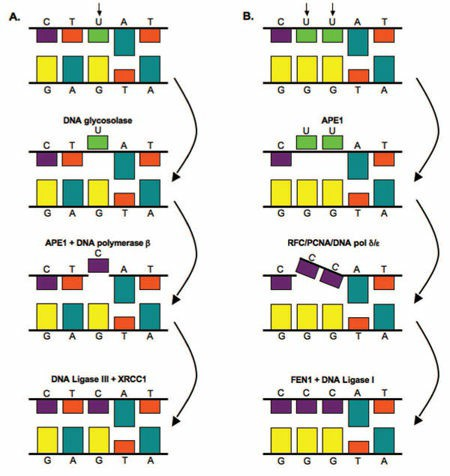
\includegraphics[width=0.5\textwidth]{Imagens/excisaodeBase.jpg}
		}%
		\caption{Via de reparo por excisão de base}
		\label{fig:excisaodeBase}
	\end{figure}

	\begin{enumerate}[label=\textcolor{CarnationPink}{\arabic*${}^\circ $}]
		\item \textcolor{DarkTurquoise}{\textbf{Reconhecimento do dano: }} O primeiro passo do BER é o reconhecimento do dano no DNA. Enzimas específicas chamadas glicosilases identificam e se ligam ao local onde a base danificada está localizada. Existem diferentes tipos de glicosilases, cada uma especializada em detectar um tipo específico de dano na base.
		\item \textcolor{DarkTurquoise}{\textbf{Remoção da base danificada: }} Após o reconhecimento do dano, a glicosilase atua removendo seletivamente a base danificada, quebrando a ligação entre a base e o açúcar do DNA. Esse processo cria um sítio apurínico ou apirimidínico (AP) no DNA, onde a base anteriormente danificada estava.
		\item \textcolor{DarkTurquoise}{\textbf{Clivagem da cadeia de açúcar-fosfato:}} Uma enzima chamada AP endonuclease reconhece o sítio AP no DNA e cliva a cadeia de açúcar-fosfato no local, removendo a base danificada. Isso resulta em uma lacuna de um ou mais nucleotídeos no DNA.
		\item \textcolor{DarkTurquoise}{\textbf{Preenchimento da lacuna:}} A lacuna deixada pela remoção da base danificada é preenchida por uma enzima chamada DNA polimerase, que adiciona novos nucleotídeos complementares à sequência do DNA. A DNA polimerase utiliza a fita intacta como modelo para sintetizar a sequência de nucleotídeos complementares. 
		\item \textcolor{DarkTurquoise}{\textbf{Selamento do reparo:}} Por fim, a enzima DNA ligase atua selando a nova sequência de nucleotídeos ao DNA, formando uma ligação fosfodiéster entre o novo segmento e a cadeia de DNA existente.
	\end{enumerate}

	    
	

\subsection*{Reparo por Excisão de Nucleotídio (NER - ``Nucleotide Excision Repair'')}

	O mecanismo de reparo por excisão de nucleotídeo (NER) é um processo celular que visa corrigir danos mais extensos no DNA, como dímeros de pirimidina e adutos de DNA. A \ref{fig:reparoExcisaoNucleotidio} apresenta um esquema de como ocorre este reparo.

	\begin{figure}[h]
		\centering
		\fcolorbox{DarkTurquoise}{white}{%
			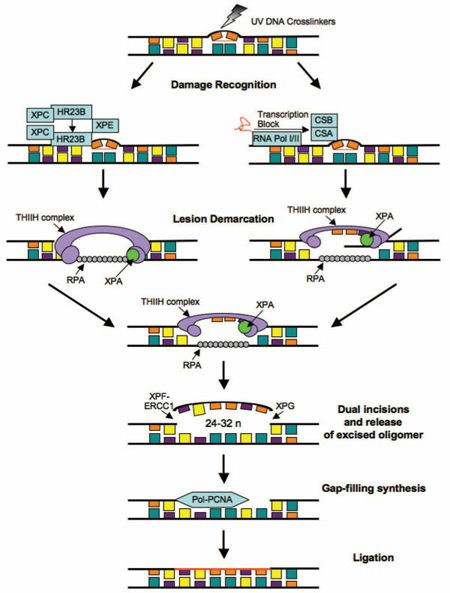
\includegraphics[width=0.5\textwidth]{Imagens/reparoExcisaoNucleotidio.jpg}
		}%
		\caption{Via de reparo por excisão do nucleotídeo}
		\label{fig:reparoExcisaoNucleotidio}
	\end{figure}

	\begin{enumerate}[label=\textcolor{CarnationPink}{\arabic*${}^\circ $}]
		\item \textcolor{DarkTurquoise}{\textbf{Reconhecimento do dano:}} O primeiro passo do NER é o reconhecimento do dano no DNA. Existem dois principais subtipos de NER: o NER global (GG-NER) e o NER de transcrição (TC-NER). O GG-NER é responsável por detectar danos no DNA em qualquer região do genoma, enquanto o TC-NER é ativado especificamente em regiões transcritas do DNA. Proteínas especializadas, como o complexo de reconhecimento de dano (DRC), reconhecem e se ligam ao dano no DNA.
		\item \textcolor{DarkTurquoise}{\textbf{Desdobramento da cadeia de DNA: }} pós o reconhecimento do dano, ocorre o desdobramento da cadeia de DNA. Proteínas, como a helicase XPB, fazem parte de complexos enzimáticos, como a RNA polimerase II, que se separam e deslocam a dupla hélice de DNA para expor o local danificado.
		\item \textcolor{DarkTurquoise}{\textbf{Remoção do segmento danificado:}}  Uma vez que o local danificado foi exposto, ocorre a remoção do segmento danificado de DNA. Enzimas conhecidas como endonucleases de excisão, como a endonuclease XPG e a endonuclease ERCC1-XPF, cortam as ligações fosfodiéster no DNA, removendo uma sequência de nucleotídeos ao redor do local danificado.
		\item \textcolor{DarkTurquoise}{\textbf{Preenchimento da lacuna:}} Com o segmento danificado removido, a lacuna resultante é preenchida por uma enzima chamada DNA polimerase. A DNA polimerase utiliza a fita intacta como modelo e adiciona novos nucleotídeos complementares à sequência de DNA.
		\item \textcolor{DarkTurquoise}{\textbf{Selagem do reparo:}} Após o preenchimento da lacuna, a enzima DNA ligase atua selando a nova sequência de nucleotídeos ao DNA existente, formando uma ligação fosfodiéster entre o novo segmento e a cadeia de DNA.
	\end{enumerate}

	As principais enzimas envolvidas no mecanismo de reparo por excisão de nucleotídeo incluem as endonucleases de excisão (como XPG e ERCC1-XPF), helicases (como XPB), DNA polimerases (como polimerase δ e polimerase ε), DNA ligase e outras proteínas reguladoras que ajudam na coordenação e na eficiência do processo de reparo.

\subsection*{Reparo de Incompatibilidade de Pares de Base (MMR - ``Mismatch Repair'')}

	O reparo de desigualdades de pares de bases, também conhecido como reparo de mismatch, apresentado na \ref{fig:mismatchReparo}, é um mecanismo celular que visa corrigir erros de pareamento de bases no DNA que ocorrem durante a replicação ou recombinação. Esses erros de pareamento resultam na formação de desigualdades de bases, ou seja, um par de bases não correspondentes na dupla hélice de DNA.

	\begin{figure}[h]
		\centering
		\fcolorbox{DarkTurquoise}{white}{%
			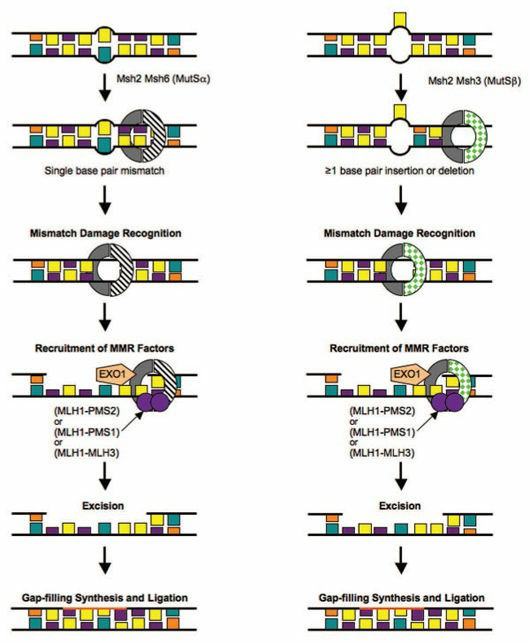
\includegraphics[width=0.5\textwidth]{Imagens/mismatchReparo.jpg}
		}%
		\caption{Reparo de incompatibilidade de Bases}
		\label{fig:mismatchReparo}
	\end{figure}

	\begin{enumerate}[label=\textcolor{CarnationPink}{\arabic*${}^\circ $}]
		\item \textcolor{DarkTurquoise}{\textbf{Reconhecimento do mismatch:}} O primeiro passo do reparo de mismatch é o reconhecimento do erro de pareamento no DNA. Complexos de proteínas especializadas, como a proteína MutS, reconhecem e se ligam às desigualdades de bases. A proteína MutS forma um complexo com outras proteínas, como a proteína MutL, para iniciar o processo de reparo.
		\item \textcolor{DarkTurquoise}{\textbf{Excisão do segmento errado:}} O primeiro passo do reparo de mismatch é o reconhecimento do erro de pareamento no DNA. Complexos de proteínas especializadas, como a proteína MutS, reconhecem e se ligam às desigualdades de bases. A proteína MutS forma um complexo com outras proteínas, como a proteína MutL, para iniciar o processo de reparo.
		\item \textcolor{DarkTurquoise}{\textbf{Remoção do segmento danificado:}} Uma vez que o sítio de clivagem foi criado, ocorre a remoção do segmento de DNA contendo a desigualdade de bases. A proteína exonuclease, como a exonuclease I, é recrutada para degradar a cadeia de DNA a partir do sítio de clivagem.
		\item \textcolor{DarkTurquoise}{\textbf{Preenchimento da lacuna:}} Com o segmento danificado removido, a lacuna resultante é preenchida pela ação da DNA polimerase e da DNA ligase. A DNA polimerase adiciona novos nucleotídeos complementares à sequência de DNA, utilizando a cadeia intacta como molde. Em seguida, a DNA ligase sela a nova sequência de nucleotídeos ao DNA existente, formando uma ligação fosfodiéster.
		\item \textcolor{DarkTurquoise}{\textbf{Controle de metilação:}} Em alguns organismos, como bactérias, o reparo de mismatch inclui um passo adicional chamado controle de metilação. Durante a replicação, as cadeias recém-sintetizadas de DNA são metiladas em bases específicas. O controle de metilação identifica a cadeia de DNA recém-sintetizada não metilada e a distingue da cadeia parental metilada, permitindo a remoção seletiva da base errada.
	\end{enumerate}

\subsection*{Reparo Crosslink}
	
	O mecanismo de reparo de crosslinks, apresentado na \ref{fig:reparoCrossLink}, é um processo celular que visa corrigir danos no DNA causados por ligações cruzadas covalentes entre as duas fitas de DNA ou entre o DNA e outras moléculas, como proteínas. Essas ligações cruzadas podem ser geradas por agentes químicos ou radiação ionizante e podem levar a quebras nas fitas de DNA, impedindo a replicação e a transcrição adequadas.

	\begin{figure}[h]
		\centering
		\fcolorbox{DarkTurquoise}{white}{%
			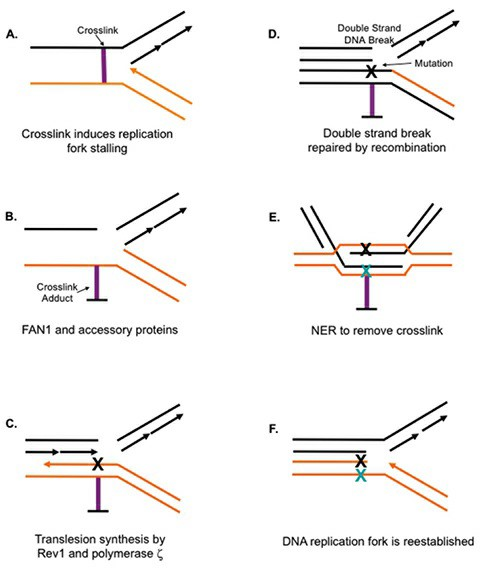
\includegraphics[width=0.5\textwidth]{Imagens/reparoCrossLink.jpg}
		}%
		\caption{Reparo crosslink}
		\label{fig:reparoCrossLink}
	\end{figure}

	\begin{enumerate}[label=\textcolor{CarnationPink}{\arabic*${}^\circ $}]
		\item \textcolor{DarkTurquoise}{\textbf{Reconhecimento do crosslink:}} O primeiro passo do reparo de crosslinks é o reconhecimento do dano no DNA. Proteínas especializadas, como a proteína de reconhecimento de crosslink (como a XPF-ERCC1), detectam a presença do crosslink e se ligam a ele. Essas proteínas atuam como sensores de danos no DNA.
		\item \textcolor{DarkTurquoise}{\textbf{Desencadeamento da resposta ao dano:}} Após o reconhecimento do crosslink, ocorre a ativação de uma cascata de sinalização para desencadear a resposta ao dano. Isso envolve a ativação de proteínas de sinalização, como as cinases ATM e ATR, que coordenam a resposta celular ao dano no DNA.
		\item \textcolor{DarkTurquoise}{\textbf{Desenrolamento da dupla hélice:}} Para permitir o acesso às ligações cruzadas no DNA, ocorre o desenrolamento da dupla hélice. Proteínas helicase, como a proteína FANCM, são recrutadas para desenrolar a estrutura do DNA nas proximidades do crosslink, expondo-o para os próximos passos do reparo.
		\item \textcolor{DarkTurquoise}{\textbf{Excisão do crosslink:}} Uma vez que o crosslink é exposto, ocorre a excisão do dano. Enzimas conhecidas como endonucleases de excisão (como a endonuclease XPF-ERCC1) são recrutadas para clivar as ligações cruzadas nas fitas de DNA, removendo o crosslink.
		\item \textcolor{DarkTurquoise}{\textbf{Reparo das quebras nas fitas de DNA:}} A remoção do crosslink geralmente resulta em quebras nas fitas de DNA. Essas quebras são reparadas através de outros mecanismos de reparo, como o reparo por recombinação homóloga ou o reparo por junção de extremidades não homólogas (NHEJ). Proteínas e enzimas envolvidas nesses mecanismos são recrutadas para reparar as quebras nas fitas de DNA, garantindo sua integridade.
	\end{enumerate}

\subsection{Reparo de Quebra de Única Fita do DNA}

	As SSBs são formadas em alta taxa durante/após irradiação e quimioterapia, mas têm pouco efeito na sobrevivência, a menos que se combinem em um DSB. 

	A poli(ADP-ribose) polimerase-1 (PARP-1) detecta o corte e sintetiza polímeros de ADP-ribose. A polimerase β geralmente está envolvida no preenchimento de lacunas, mas outras polimerases podem estar envolvidas. A ligação do DNA após o reparo de patch curto é realizada pela Ligase 3 em coordenação com uma proteína scaffold (XRCC1), e a ligação após o reparo de patch longo é concluída pela Ligase 1.


\subsection{Reparo das Quebras na Dupla Fita do DNA}

	As quebras na dupla fita do DNA são as formas mais graves de danos no DNA, pois podem levar à perda de informações genéticas ou rearranjos cromossômicos. Para reparar essas quebras, as células utilizam dois principais mecanismos de reparo: reparo por recombinação homóloga (HR) e reparo por junção de extremidades não homólogas (NHEJ), como mostra a \ref{fig:reparoQuebraDupla}. 

	\begin{figure}
		\centering
		\fcolorbox{DarkTurquoise}{white}{%
			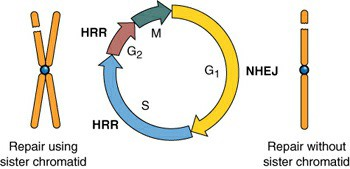
\includegraphics[width=0.5\textwidth]{Imagens/reparoQuebraDupla.jpg}
		}%
		\caption{Reparos das Quebras na dupla fita do DNA com relação as etapas do ciclo celular}
		\label{fig:reparoQuebraDupla}
	\end{figure}

\subsection*{Reparo por Recombinação Homóloga (HR - ``Homologous recombination'')}

	O reparo por recombinação homóloga (HR) (\ref{fig:recombinacaoHomologa}) é um mecanismo complexo e preciso de reparo de quebras na dupla fita do DNA. Ele utiliza uma sequência de DNA homóloga como molde para a restauração da sequência original.

	\begin{figure}
		\centering
		\fcolorbox{DarkTurquoise}{white}{%
			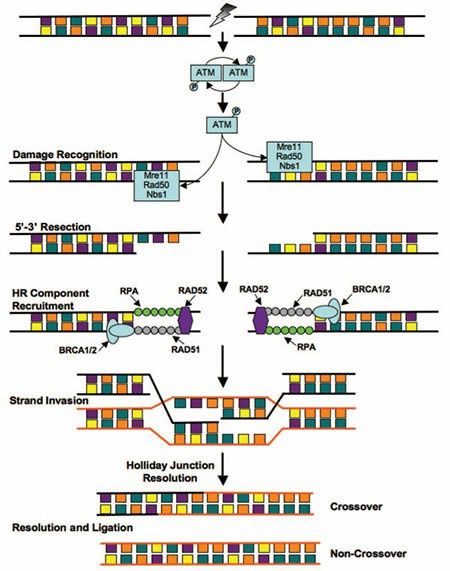
\includegraphics[width=0.5\textwidth]{Imagens/recombinacaoHomologa.jpg}
		}%
		\caption{Via de reparo por recombinação homóloga}
		\label{fig:recombinacaoHomologa}
	\end{figure}

	\begin{enumerate}[label=\textcolor{CarnationPink}{\arabic*${}^\circ $}]
		\item \textcolor{DarkTurquoise}{\textbf{Reconhecimento da quebra:}} Proteínas sensoras de danos, como a proteína MRN (Mre11-Rad50-Nbs1), reconhecem as quebras na dupla fita do DNA. O complexo MRN se liga às extremidades da quebra e recruta outras proteínas envolvidas no reparo. 
		\item \textcolor{DarkTurquoise}{\textbf{Processamento das extremidades da quebra:}} A proteína MRN processa as extremidades da quebra, removendo quaisquer danos ou terminações prejudiciais. O complexo MRN também recruta e ativa a cinase do ponto de verificação do dano ao DNA (ATM), que fosforila várias proteínas envolvidas no reparo. A HR geralmente é iniciada pela fosforilação do BRCA1 pela ATM, que se une ao PARP e ao complexo MRN no local da DSB (o Nbs1 fosforilado é necessário para a redistribuição do MRN nos locais dos DSBs). A histona H2AX é fosforilada por ATM e torna-se $\gamma$-H2AX, que então forma focos na cromatina nas proximidades do DSB. Depois que os DSBs são induzidos, o CtIP é fosforilado por ATM e ubiquitinado por BRCA1, resultando em sua ativação e recrutamento para as extremidades do DNA, comprometendo as células para a via HR. CtIP e o complexo MRN iniciam a ressecção de DSB (Mre11 pode funcionar como uma endo e exonuclease) por meio da clivagem endonucleolítica e do processamento de extremidades quebradas.
		\item \textcolor{DarkTurquoise}{\textbf{Formação do complexo de pré-invasão:}} A proteína RPA (replication protein A) se liga às extremidades da quebra, evitando que as fitas de DNA se recombinem prematuramente. A proteína RAD52 se liga ao RPA e forma o complexo de pré-invasão, que é essencial para a posterior invasão do DNA homólogo.
		\item \textcolor{DarkTurquoise}{\textbf{Remoção do RPA e recrutamento do RAD51:}}  O complexo de pré-invasão promove a remoção do RPA e recruta a proteína RAD51. O RAD51 forma filamentos nucleoproteicos, que são estruturas helicoidais compostas por RAD51 e DNA de fita simples. Rad51 é a chave para o HRR, pois participa da troca de fitas, facilitando a invasão do DNA danificado no DNA homólogo.
		\item \textcolor{DarkTurquoise}{\textbf{Invasão do DNA homólogo:}} o Rad54 desenrola o DNA, proporcionando acessibilidade e, junto com o BRCA2, coordena a localização, alinhamento e carregamento dos complexos proteicos Rad51. O filamento de RAD51 invade o DNA homólogo intacto, procurando por uma sequência homóloga para emparelhar. O pareamento ocorre entre a fita danificada e a fita homóloga no DNA intacto, formando uma estrutura de pareamento de bases.
		\item \textcolor{DarkTurquoise}{\textbf{Síntese de DNA e formação de junção de Holliday:}} Enzimas de replicação de DNA, como a DNA polimerase, sintetizam nova fita de DNA usando a fita intacta como molde. Durante a síntese de DNA, ocorre a troca de fitas entre as moléculas de DNA, levando à formação de uma junção de Holliday.
		\item \textcolor{DarkTurquoise}{\textbf{Resolução da junção de Holliday:}} A junção de Holliday é resolvida por enzimas resolvases, como a resolvase de junção de Holliday (RuvC) em bactérias. A resolvase corta as hélices de DNA cruzadas da junção de Holliday, permitindo a separação das moléculas de DNA recombinadas.
		\item \textcolor{DarkTurquoise}{\textbf{Preenchimento das lacunas e selagem:}} Após a resolução da junção de Holliday, ocorre o preenchimento das lacunas restantes com a DNA polimerase e a DNA ligase. A DNA polimerase sintetiza o DNA ausente e a DNA ligase sela as extremidades, restaurando a integridade da dupla fita.
	\end{enumerate}

	HR é a forma predominante de reparo do DNA durante a fase S tardia e G2, quando as cromátides-irmãs estão disponíveis para permitir que um trecho de algumas centenas de pares de bases de homologia de sequência seja usado como modelo para restaurar a sequência de DNA quebrada. HR é relativamente livre de erros. 
	
	Mutações nos genes ATM, MRE11 e NBS1 resultam em síndromes associadas ao aumento da radiossensibilidade e predisposição ao câncer. As mutações BRCA1/2 são responsáveis por síndromes hereditárias de câncer de mama e ovário.

\subsection*{Reparo por Junção de Extremidades Não Homólogas (NHEJ)}

	O reparo por junção de extremidades não homólogas (\ref{fig:recombinacaoNaoHomologa}) é um mecanismo de reparo de quebras na dupla fita do DNA que ocorre principalmente durante as fases G0 e G1 do ciclo celular pois não existem cromátides-irmãs, Também pode ocorrer nas fases S e G2, embora a HR seja a principal. Ao contrário do reparo por recombinação homóloga, o NHEJ não requer uma sequência homóloga como molde e, portanto, pode ser mais rápido, mas também mais propenso a erros, uma vez que a sequência de DNA original seria restaurável apenas se duas extremidades rombas pudessem ser religadas sem perda de qualquer informação genética perto dos locais de quebra; Isto pode levar à mutação ou morte celular.
	



	\begin{figure}[h]
		\centering
		\fcolorbox{DarkTurquoise}{white}{%
			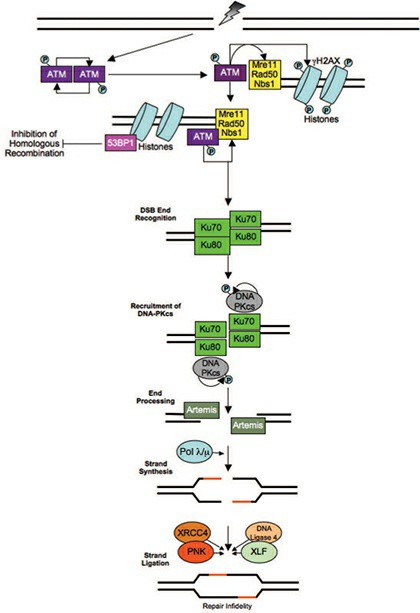
\includegraphics[width=0.5\textwidth]{Imagens/recombinacaoNaoHomologa.jpg}
		}%
		\caption{Via de reparo por junção de extremidades não homólogas}
		\label{fig:recombinacaoNaoHomologa}
	\end{figure}

	\begin{enumerate}[label=\textcolor{CarnationPink}{\arabic*${}^\circ $}]
		\item \textcolor{DarkTurquoise}{\textbf{Reconhecimento da quebra:}} A indução de DSB resulta no recrutamento do heterodímero Ku70/Ku80 para o sítio DSB para ligar as extremidades livres. Essas proteínas sensoras de danos reconhecem as quebras na dupla fita do DNA de modo que a proteína Ku se liga às extremidades da quebra e atua como um marcador para recrutar outras proteínas envolvidas no reparo.
		\item \textcolor{DarkTurquoise}{\textbf{Ligação do complexo proteico:}} O complexo proteico formado por Ku recruta outras proteínas, incluindo a DNA-PKcs (cinase dependente de DNA-PK), formando o complexo de reparo por NHEJ. Ocorre fosforilação e ativação de Artemis por DNA-PK, permitindo que Artemis funcione como uma exonuclease no processamento da lesão.
		\item \textcolor{DarkTurquoise}{\textbf{Processamento das extremidades da quebra:}} As extremidades da quebra são processadas pela atividade de nucleases, que removem quaisquer danos ou terminações prejudiciais.
		\item \textcolor{DarkTurquoise}{\textbf{Remoção de nucleotídeos:}} Em algumas situações, é necessária a remoção de nucleotídeos em excesso nas extremidades da quebra para permitir a ligação das extremidades. Isso é realizado por nucleases específicas, como a Artemis.
		\item \textcolor{DarkTurquoise}{\textbf{Ligação das extremidades:}} As extremidades processadas são trazidas em proximidade pelo complexo de reparo por NHEJ e ligadas pela atividade da ligase IV, que forma uma ligação fosfodiéster entre as extremidades.
		\item \textcolor{DarkTurquoise}{\textbf{Selagem da ligação:}}  A ligação fosfodiéster formada pela ligase IV é selada pela atividade da XRCC4 (proteína de reparo do DNA cruzada por radiação 4) e outros fatores de ligação.
		\item \textcolor{DarkTurquoise}{\textbf{Finalização do reparo:}} Após a selagem da ligação, o reparo por NHEJ é concluído. No entanto, esse processo pode resultar em alterações na sequência do DNA, como pequenas deleções ou inserções, devido à remoção de nucleotídeos ou processamento impreciso das extremidades da quebra.
	\end{enumerate}


	Existe uma via delecional alternativa (A-NHEJ), que requer microhomologia para unir as extremidades dos DSBs com pequenas deleções. A via A-NHEJ é independente de Ku, mas requer DNA ligase III e PARP I. 
	
	As DSBs são o principal mecanismo de morte celular induzida por radiação, então qualquer defeito no reparo de DSB pode aumentar a sensibilidade à radiação. A \ref{fig:danoEReparonoDna} apresenta os tipos de dano e seus respectivos reparos, onde o dano ao DNA pode ser reparado por uma das diferentes vias de reparo, dependendo do tipo de dano e da fase do ciclo celular que ocorre esse dano.

	\begin{figure}[h]
		\centering
		\fcolorbox{DarkTurquoise}{white}{%
			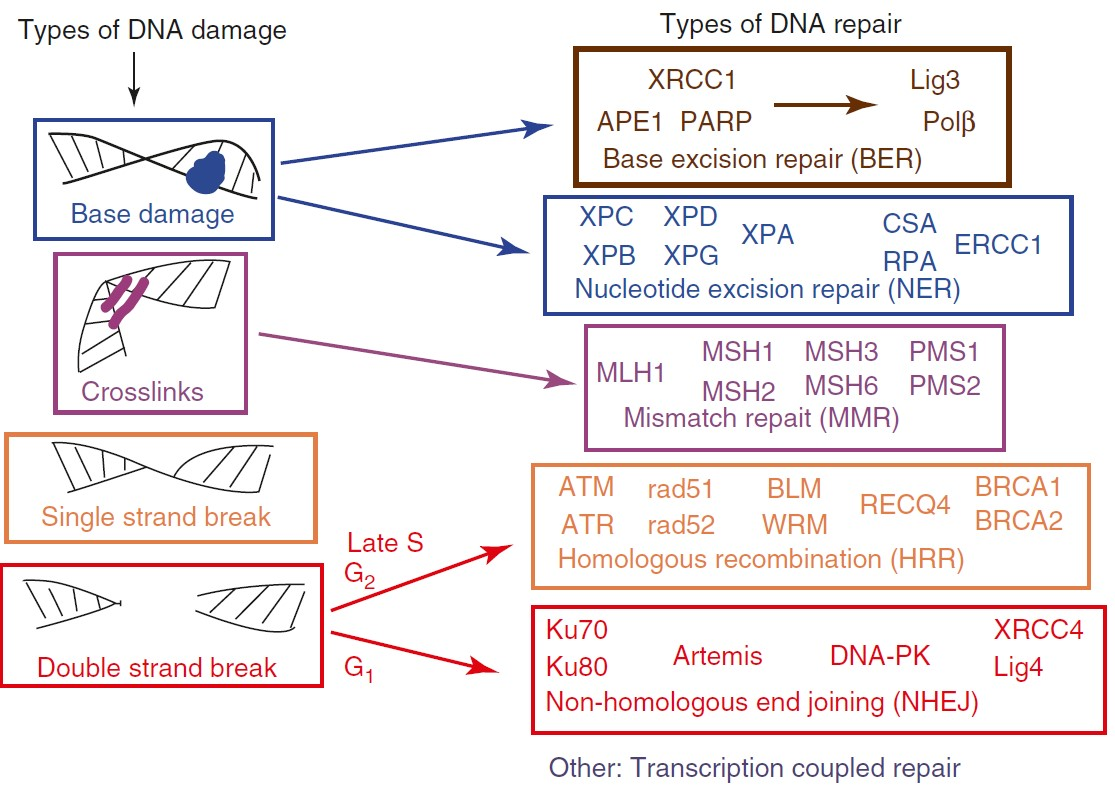
\includegraphics[width=0.8\textwidth]{Imagens/danoEReparonoDna.jpg}
		}%
		\caption{Vias de reparo do DNA}
		\label{fig:danoEReparonoDna}
	\end{figure}

\section{Doenças Genéticas Humanas Devido à Deficiências no Reparo do DNA}

	Existem diferentes doenças associadas à falhas nos mecanismos de reparo do DNA e muitas delas estão associadas a predispocição ao câncer.

	\begin{itemize}[label=\textcolor{CarnationPink}{$\blacktriangleright$}]
		\item \textcolor{DarkTurquoise}{\LobsterTwo\Large\textbf{Deficiências no Reparo por Recisão do Nucleotídio}}
		\begin{itemize}[label=\textcolor{CarnationPink}{$\star$}]
			\item \textcolor{MediumOrchid}{\large\textbf{Xeroderma Pigmentoso (gene XP):}} 
			
			O Xeroderma Pigmentoso é uma doença genética rara e hereditária que afeta a capacidade do organismo de reparar o DNA danificado pela exposição à radiação ultravioleta (UV) do sol e outras fontes. Essa condição é caracterizada pela extrema sensibilidade à luz solar, desenvolvimento de eritema (vermelhidão) na pele após exposição mínima ao sol e o aparecimento de lesões cutâneas, como manchas, bolhas, úlceras e pigmentação irregular.
			
			\

			A principal causa do xeroderma pigmentoso é uma mutação genética em um dos vários genes relacionados ao reparo do DNA. Esses genes estão envolvidos no reparo das lesões causadas pela radiação UV, como dímeros de pirimidina, que são ligações anormais entre as bases pirimidínicas (timina e citosina) no DNA.

			\

			Devido à deficiência no reparo do DNA, as pessoas com XP têm um risco significativamente aumentado de desenvolver câncer de pele, principalmente carcinomas de células escamosas e melanomas. Além disso, também podem apresentar alterações neurológicas, como atraso no desenvolvimento, perda de audição, distúrbios neurológicos e déficits cognitivos.
			
			\

			Portanto o Xeroderma Pigmentoso apresenta uma fotossensibilidade e risco muito alto de câncer de pele. E embora seja ultrassensível aos raios ultravioleta, não é radiossensível.
			
			\

			\item \textcolor{MediumOrchid}{\large\textbf{Síndrome de Cockayne (genes CSA/CSB):}}
			
			A sindrome de Cockayne é uma doença genética rara e progressiva que afeta o desenvolvimento e o envelhecimento precoce de uma pessoa. É caracterizada por um conjunto específico de características clínicas, incluindo crescimento retardado, anormalidades faciais, sensibilidade à luz solar, perda de audição, problemas neurológicos e envelhecimento acelerado.
			
			\

			A síndrome de Cockayne é causada por mutações em genes específicos que estão envolvidos na reparação do DNA danificado. Esses genes são responsáveis por corrigir os danos acumulados no DNA, incluindo aqueles causados pela exposição à radiação ultravioleta. Como resultado da deficiência no reparo do DNA, ocorre o acúmulo de danos e mutações, levando ao envelhecimento celular prematuro e disfunção de vários sistemas no organismo.
			
			\

			A Sindrome de Cockayne é fótossensível mas não oferece risco de câncer e nem é sensível a radiação ionizante.
		\end{itemize}
		
		\

		\item \textcolor{DarkTurquoise}{\LobsterTwo\Large\textbf{Deficiências no Reparo Mismacht}}
		\begin{itemize}[label=\textcolor{CarnationPink}{$\star$}]
			\item \textcolor{MediumOrchid}{\large\textbf{Sindrome de Lynch:}} 
			
			A síndrome de Lynch, também conhecida como câncer colorretal hereditário não poliposo (HNPCC, do inglês "hereditary non-polyposis colorectal cancer"), é uma doença genética hereditária que aumenta significativamente o risco de desenvolver câncer colorretal e outros tipos de câncer, como câncer de endométrio, ovário, estômago, intestino delgado, ureter, pelve renal e trato biliar.
			
			\

			A síndrome de Lynch é causada por mutações em genes que estão envolvidos na correção de erros no DNA durante a replicação celular. As mutações mais comuns estão nos genes MLH1, MSH2, MSH6 e PMS2, que são responsáveis pela reparação de erros de pareamento de bases durante a replicação do DNA. Esses erros, conhecidos como instabilidade de microssatélites, podem ocorrer com maior frequência nas células com mutações nos genes da síndrome de Lynch.

			\

			Normalmente, esses genes ajudam a corrigir erros no pareamento de bases durante a replicação do DNA, garantindo a integridade genética. No entanto, quando ocorrem mutações nesses genes, a capacidade do organismo de reparar corretamente o DNA danificado é comprometida, levando a um aumento na acumulação de erros genéticos ao longo do tempo.

			\

			A síndrome de Lynch é transmitida de forma autossômica dominante, o que significa que um único gene defeituoso herdado de um dos pais é suficiente para aumentar o risco de desenvolver câncer. Portanto, indivíduos que têm um parente de primeiro grau com síndrome de Lynch têm 50\% de chance de herdar a mutação genética.

			\

			Portanto a Sindrome de Lynch tem um risco extremamente alto de causar cancer coloretal. Esta sindrome não é radiossensível mas pode ser hipersensível a quimioterapia.

		\end{itemize}

		\item \textcolor{DarkTurquoise}{\LobsterTwo\Large\textbf{Deficiências na Recombinação Homóloga}}
		\begin{itemize}[label=\textcolor{CarnationPink}{$\star$}]
			\item \textcolor{MediumOrchid}{\large\textbf{Síndrome hereditária de câncer de mama e ovário:}} 
			A síndrome hereditária de câncer de mama e ovário é uma condição genética que aumenta o risco de desenvolver câncer de mama e câncer de ovário em mulheres. É causada por mutações em genes específicos que estão envolvidos no reparo do DNA e na supressão de tumores.

			\

			Os dois principais genes associados à síndrome hereditária de câncer de mama e ovário são o BRCA1 (Breast Cancer Gene 1) e o BRCA2 (Breast Cancer Gene 2). Esses genes são responsáveis pela produção de proteínas que desempenham um papel crucial na manutenção da integridade do DNA, reparação de danos e regulação do crescimento celular.

			\

			As mutações nos genes BRCA1 e BRCA2 aumentam significativamente o risco de desenvolver câncer de mama e câncer de ovário. Estima-se que mulheres com uma mutação no BRCA1 têm cerca de 40\% a 80\% de chance de desenvolver câncer de mama ao longo da vida, e cerca de 20\% a 60\% de chance de desenvolver câncer de ovário. Para as mulheres com mutações no BRCA2, o risco estimado é de cerca de 40\% a 70\% para câncer de mama e de 10\% a 30\% para câncer de ovário.

			\

			As mutações nos genes BRCA1 e BRCA2 podem ser herdadas de um dos pais. Quando uma pessoa herda uma mutação em um desses genes, suas células estão mais propensas a acumular danos no DNA ao longo do tempo. Isso pode levar a mutações adicionais em genes supressores de tumores e aumentar a probabilidade de desenvolver câncer.

			\

			As mulheres o são aconselhadas a fazer testes genéticos para identificar mutações nos genes BRCA1 e BRCA2 se tiverem uma história familiar significativa de câncer de mama, câncer de ovário ou outros tipos de câncer relacionados à síndrome.

			\

			Apesar do defeito no reparo do DNA, os pacientes BRCA1/2 não são extremamente radiossensíveis.

		\end{itemize}
		\item \textcolor{DarkTurquoise}{\LobsterTwo\Large\textbf{Deficiências em Múltiplas vias de Reparo}}
		\begin{itemize}[label=\textcolor{CarnationPink}{$\star$}]
			\item \textcolor{MediumOrchid}{\large\textbf{Ataxia Telangiectasia:}}
			
			A Ataxia Telangiectasia (AT) é uma doença genética rara e progressiva que afeta múltiplos sistemas do corpo. É caracterizada por problemas de coordenação motora, comprometimento do sistema imunológico, telangiectasias (dilatação dos vasos sanguíneos) e predisposição a infecções respiratórias recorrentes. Além disso, os indivíduos com AT têm um risco significativamente aumentado de desenvolver câncer, especialmente leucemia e linfoma.

			\

			A AT é causada por mutações no gene ATM (Ataxia Telangiectasia Mutated), que está envolvido na regulação da resposta ao dano no DNA e na reparação de quebras de dupla fita do DNA. O gene ATM produz uma proteína que desempenha um papel essencial na sinalização de danos no DNA e na ativação de mecanismos de reparo celular.

			\

			As mutações no gene ATM resultam em uma deficiência ou ausência da proteína ATM funcional. Isso leva a uma incapacidade das células do organismo em reparar corretamente o DNA danificado, o que leva ao acúmulo de danos no DNA ao longo do tempo. Esse acúmulo de danos no DNA afeta negativamente a função celular e leva aos sintomas e características da AT.

			\

			A ausência da proteína ATM funcional também causa instabilidade genômica, ou seja, o DNA se torna mais suscetível a erros de replicação e rearranjos cromossômicos, o que pode contribuir para a predisposição ao desenvolvimento de câncer. Além disso, é extremamente radiossensível.

			\

			\item \textcolor{MediumOrchid}{\large\textbf{Transtorno tipo ataxia-telangiectasia:}}
			
			O Transtorno Tipo Ataxia-Telangiectasia, também conhecido como AT-like disorder (ATLD), é uma condição genética relacionada à Ataxia Telangiectasia, mas causada por mutações em um gene diferente chamado MRE11A. O gene MRE11A é responsável pela produção de uma proteína chamada MRE11, que também desempenha um papel importante na reparação do DNA e na resposta ao dano genômico.

			\

			As mutações no gene MRE11A resultam em uma deficiência ou alteração funcional da proteína MRE11, afetando negativamente a capacidade das células de reparar corretamente o DNA danificado. Isso leva a sintomas semelhantes aos da Ataxia Telangiectasia, como problemas de coordenação motora, imunodeficiência e predisposição ao câncer, embora geralmente em menor gravidade do que na AT. Porém, a ATLD também é extremamente radiossensível.

			\

			\item \textcolor{MediumOrchid}{\large\textbf{Síndrome de quebra de Nijmegen:}}
			
			A Síndrome de Quebra de Nijmegen, também conhecida como Síndrome de Nijmegen Breakage (NBS), é uma doença genética rara e hereditária caracterizada por defeitos no reparo do DNA e instabilidade cromossômica. É uma condição autossômica recessiva, o que significa que ambos os pais devem transmitir uma cópia do gene mutado para que a doença se manifeste. 

			\

			A NBS é causada por mutações no gene Nbs1 (Nibrin), que é responsável pela produção da proteína nibrina. A nibrina é uma proteína essencial para a integridade do genoma e desempenha um papel crucial no reparo do DNA de quebras de dupla fita. O gene Nbs1 está localizado no cromossomo 8q21 e contém 16 éxons.

			\

			As mutações no gene Nbs1 resultam na produção de uma proteína nibrina não funcional ou em níveis reduzidos de proteína. Isso compromete a capacidade das células em reparar corretamente o DNA danificado, especialmente as quebras de dupla fita do DNA. Como resultado, ocorre instabilidade genômica, com danos no DNA acumulando-se ao longo do tempo. Também de trata de uma síndrome extremamente radiossensível.

			\

			\item \textcolor{MediumOrchid}{\large\textbf{Síndrome de Li-Fraumeni:}}
			
			A Síndrome de Li-Fraumeni é uma síndrome hereditária rara e de predisposição ao câncer. Ela foi descrita pela primeira vez em 1969 por Frederick Li e Joseph Fraumeni. A síndrome é caracterizada por uma predisposição aumentada ao desenvolvimento de vários tipos de câncer em indivíduos afetados e seus familiares.

			\

			A Síndrome de Li-Fraumeni é causada por mutações no gene TP53, também conhecido como "guardião do genoma". O gene TP53 está localizado no braço curto do cromossomo 17 (17p13.1) e é responsável pela produção da proteína p53. A proteína p53 é um fator de transcrição que desempenha um papel crucial na regulação do ciclo celular, reparo do DNA, indução da apoptose (morte celular programada) e supressão tumoral.

			\

			As mutações no gene TP53 levam à produção de uma forma não funcional ou alterada da proteína p53. Como resultado, a proteína p53 não é capaz de exercer adequadamente suas funções reguladoras no genoma, o que leva a uma maior susceptibilidade ao desenvolvimento de câncer. As mutações no gene TP53 estão associadas a uma variedade de tumores, incluindo sarcomas, tumores cerebrais, câncer de mama, câncer colorretal, câncer de pulmão, entre outros.

			\

			A Síndrome de Li-Fraumeni é herdada de forma autossômica dominante, o que significa que um único alelo mutado do gene TP53 é suficiente para aumentar o risco de desenvolver câncer. Isso significa que os indivíduos afetados têm uma chance de 50\% de transmitir a mutação para seus filhos.

			\

			Portanto, está síndrome está relacionadas a numerosos cânceres em uma idade jovem e é um tanto radiossensível e com taxa muito alta de causar malignidades radio-induzidas.

		\end{itemize}
		\item \textcolor{DarkTurquoise}{\LobsterTwo\Large\textbf{Outros distúrbios associados à radiossensibilidade.}}
		
		As síndromes citadas abaixo são todas radiossensíveis, ou seja, indivíduos portadores destas doenças poderão estar mais suscetíveis aos danos radio-induzidos; E estas síndromes podem ou não estar realcionadas a uma pré-disposição para o desenvolvimento de câncer.
		
		\

		\begin{itemize}[label=\textcolor{CarnationPink}{$\star$}]
			\item \textcolor{MediumOrchid}{\large\textbf{Síndrome nevoide basocelular:}} 
			
			A Síndrome Nevoide Basocelular, também conhecida como Síndrome de Gorlin-Goltz, é uma doença genética rara e hereditária que afeta múltiplos sistemas do corpo. Ela é caracterizada por um conjunto de manifestações clínicas, incluindo o desenvolvimento de múltiplos tumores basocelulares da pele, anomalias esqueléticas, cistos odontogênicos e outras características distintivas.

			\

			A síndrome é causada por mutações no gene PTCH1 (Proteína Patched 1), localizado no braço longo do cromossomo 9 (9q22.3). O gene PTCH1 codifica a proteína Patched 1, que desempenha um papel fundamental na via de sinalização Hedgehog, uma via importante para o desenvolvimento e crescimento celular adequados.

			\

			As mutações no gene PTCH1 resultam em uma proteína Patched 1 não funcional ou com atividade reduzida. Isso leva a uma ativação descontrolada da via Hedgehog, resultando em um aumento na proliferação celular e desenvolvimento de tumores basocelulares da pele. Esses tumores são geralmente benignos, mas podem se tornar localmente invasivos se não forem tratados precocemente.

			\

			Além dos tumores basocelulares, a Síndrome Nevoide Basocelular pode apresentar outras manifestações clínicas, incluindo anomalias esqueléticas, como costelas adicionais ou ausentes, deformidades da coluna vertebral, mandíbula proeminente e craniossinostose (fechamento prematuro das suturas cranianas). Também pode haver cistos odontogênicos na mandíbula, tumores cerebrais, como meduloblastomas, e anomalias oculares, como catarata e estrabismo.

			\

			\item \textcolor{MediumOrchid}{\large\textbf{Anemia de Fanconi:}}
			
			A Anemia de Fanconi é uma doença genética rara e hereditária que afeta a medula óssea e diversos sistemas do corpo. Ela é caracterizada por defeitos na reparação do DNA, o que leva a uma maior susceptibilidade a danos no DNA e ao desenvolvimento de anomalias congênitas, distúrbios hematológicos e um aumento no risco de desenvolver câncer.

			\

			A Anemia de Fanconi ocorre devido a mutações em um conjunto de genes que são responsáveis pela função correta do complexo de proteínas Fanconi. Até o momento, foram identificados mais de 20 genes associados à doença, sendo os genes FANCA, FANCB, FANCC, FANCD1/BRCA2, FANCD2, FANCE, FANCF, FANCG, FANCI e FANCJ os mais comumente afetados. Esses genes desempenham um papel crucial na reparação do DNA e na manutenção da estabilidade genômica.

			\

			A função do complexo de proteínas Fanconi é detectar e reparar danos no DNA, especialmente danos nas fitas de DNA dupla. Em indivíduos com Anemia de Fanconi, as mutações nos genes relacionados levam a uma disfunção no complexo de proteínas, resultando em um defeito na reparação do DNA. Isso aumenta a fragilidade cromossômica e a susceptibilidade a quebras no DNA, levando a uma série de problemas de saúde associados à síndrome.

			\

			Os sintomas e as manifestações clínicas da Anemia de Fanconi variam amplamente, mas podem incluir anemia aplástica, anomalias congênitas, baixa estatura, distúrbios do trato genital, anomalias esqueléticas, predisposição a infecções, insuficiência de medula óssea e um risco aumentado de desenvolver leucemia e tumores sólidos.

			\

			\item \textcolor{MediumOrchid}{\large\textbf{Síndrome de Gardner:}}
			
			A Síndrome de Gardner é uma condição genética rara que faz parte de um espectro de doenças chamadas de polipose adenomatosa familiar (FAP). É caracterizada pela presença de múltiplos pólipos no cólon, além de manifestações clínicas adicionais, como tumores ósseos, cistos sebáceos, fibromas e outras anomalias.

			\

			A síndrome ocorre devido a mutações no gene APC (Adenomatous Polyposis Coli), localizado no braço longo do cromossomo 5 (5q22.2). O gene APC é responsável por codificar a proteína APC, que regula o crescimento e a divisão celular e atua como um supressor tumoral. As mutações no gene APC resultam em uma proteína APC defeituosa ou ausente, levando ao desenvolvimento de múltiplos pólipos no cólon e ao aumento do risco de câncer colorretal. Os pólipos que se desenvolvem na Síndrome de Gardner são principalmente adenomas, que são crescimentos benignos no revestimento do cólon. No entanto, se não forem tratados, esses pólipos podem se tornar cancerosos ao longo do tempo. 

			\

			\item \textcolor{MediumOrchid}{\large\textbf{Síndrome de Usher:}}
			
			A Síndrome de Usher é uma doença genética rara que afeta a audição e a visão. Ela é caracterizada por perda auditiva ou surdez desde o nascimento ou na infância, além de problemas progressivos na visão, como retinose pigmentar (degeneração progressiva da retina) e comprometimento do campo visual.

			\

			A síndrome ocorre devido a mutações em vários genes diferentes, mas os genes mais comumente associados à Síndrome de Usher são o MYO7A, USH2A, CDH23, PCDH15, USH1C, USH1G e GPR98. Esses genes estão envolvidos no desenvolvimento e funcionamento adequado das células ciliadas sensoriais no ouvido interno e nas células fotoreceptoras da retina. As mutações nesses genes afetam a estrutura e a função dessas células, resultando em perda auditiva e problemas de visão.

			\

			\item \textcolor{MediumOrchid}{\large\textbf{Síndrome de Werner:}}
			
			A Síndrome de Werner, também conhecida como progeria adulta, é uma doença genética rara que causa envelhecimento precoce e acelerado. Ela é caracterizada por um conjunto de sintomas, incluindo perda de peso, cabelos grisalhos e rarefação, pele enrugada, problemas cardiovasculares, catarata, diabetes mellitus, osteoporose e risco aumentado de câncer.

			\

			A síndrome ocorre devido a mutações no gene WRN (Werner Syndrome RecQ Like Helicase), localizado no braço curto do cromossomo 8 (8p12). O gene WRN é responsável por codificar uma helicase do tipo RecQ, uma enzima envolvida na manutenção e reparo do DNA. As mutações no gene WRN levam à produção de uma proteína WRN defeituosa ou ausente, o que resulta em uma série de disfunções celulares e aceleração do envelhecimento.

			\

			\item \textcolor{MediumOrchid}{\large\textbf{Síndrome de Bloom:}}
			
			A Síndrome de Bloom, também conhecida como Síndrome de Bloom-Torre-Machacek, é uma doença genética rara caracterizada por um crescimento lento e anormal, predisposição a infecções recorrentes, alta incidência de câncer e sensibilidade à luz solar.

			\

			Essa síndrome é causada por mutações no gene BLM (Bloom Syndrome RecQ Like Helicase), localizado no braço longo do cromossomo 15 (15q26.1). O gene BLM codifica uma enzima chamada helicase BLM, que está envolvida na manutenção e reparo do DNA. As mutações no gene BLM levam à produção de uma proteína BLM defeituosa ou ausente, resultando em disfunções no reparo do DNA e instabilidade genômica.

			\

			\item \textcolor{MediumOrchid}{\large\textbf{Síndrome de Down:}}
			
			A Síndrome de Down, também conhecida como trissomia do cromossomo 21, é uma condição genética que ocorre devido à presença de uma cópia extra do cromossomo 21. Essa alteração genética resulta em características físicas distintas e pode levar a atrasos no desenvolvimento intelectual e em outras áreas.

			\

			Normalmente, os seres humanos possuem duas cópias do cromossomo 21, mas em indivíduos com Síndrome de Down, ocorre uma cópia adicional total ou parcial do cromossomo 21. Essa alteração cromossômica ocorre espontaneamente durante a formação dos gametas (óvulos ou espermatozoides) ou na concepção. A Síndrome de Down não está relacionada a um único gene específico, mas sim a uma alteração cromossômica. A presença da cópia extra do cromossomo 21 leva a uma expressão alterada de vários genes localizados nesse cromossomo, o que resulta nas características observadas na síndrome.

		\end{itemize}
	\end{itemize}

\section{Letalidade Sintética}

	O conceito de letalidade sintética está relacionado à interação entre duas ou mais mutações genéticas que, isoladamente, podem não ser letais para a célula, mas quando ocorrem juntas, resultam em morte celular ou comprometimento significativo da viabilidade.

	No contexto do reparo do DNA, a letalidade sintética refere-se à situação em que a combinação de mutações em genes envolvidos em diferentes vias de reparo do DNA resulta em uma sensibilidade aumentada ao dano no DNA. Isso ocorre porque as células cancerígenas geralmente têm deficiências em vias de reparo do DNA, tornando-as mais dependentes de outras vias compensatórias para manter a integridade genômica. Portanto, quando uma célula cancerígena possui mutações em duas ou mais vias de reparo do DNA, a letalidade sintética ocorre e a célula é incapaz de reparar eficientemente o dano no DNA, levando à morte celular seletiva. 

	A letalidade sintética é um princípio importante no desenvolvimento de terapias anticâncer direcionadas. A ideia é explorar as vulnerabilidades específicas das células cancerígenas com base nas mutações em vias de reparo do DNA, de modo a direcionar essas células com maior precisão, minimizando os efeitos colaterais nos tecidos normais. Os inibidores de vias específicas de reparo do DNA podem ser utilizados em combinação com outras terapias, como quimioterapia ou radioterapia, para promover a letalidade sintética nas células tumorais. No entanto, algumas células cancerígenas podem adquirir mecanismos de resistência e reparo do DNA que diminuem sua sensibilidade à radioterapia.

	Um exemplo bem conhecido de letalidade sintética no reparo do DNA é a combinação de mutações no gene BRCA1 ou BRCA2 com inibidores da enzima PARP (poli(ADP-ribose) polimerase).  As células com mutações nessas proteínas estão deficientes na via de reparo do DNA por recombinação homóloga. O uso de inibidores de PARP nessas células leva a um acúmulo de danos no DNA, resultando em letalidade sintética e morte celular seletiva nas células cancerígenas, enquanto as células normais com vias de reparo do DNA intactas são menos afetadas. 
	
	Já no contexto da radioterapia, se uma célula cancerígena tem uma deficiência na via de reparo por recombinação homóloga, como mutações nos genes BRCA1 ou BRCA2, e a radioterapia causa danos no DNA que são reparados principalmente por essa via, a célula cancerígena terá dificuldade em reparar esses danos e será mais suscetível à morte celular induzida pela radiação. 
	
	Portanto a combinação de radioterapia com agentes quimioterápicos que visam vias de reparo específicas, explorando a letalidade sintética, também pode ser utilizada para aumentar a eficácia do tratamento ao mesmo tempo que minimiza os danos nas células normais.

\bibliography{ref.bib}
\end{document}